\documentclass[uplatex, titlepage, fontsize=10pt, paper=a4paper]{jsarticle}
\usepackage[top=20truemm,bottom=20truemm,left=20truemm,right=20truemm]{geometry}
% 数式
\usepackage{amsmath,amsfonts}
\usepackage{mathtools}
\usepackage{bm}
% 画像
\usepackage[dvipdfmx]{graphicx}
\usepackage{wrapfig}

\usepackage{autobreak}
\usepackage[subrefformat=parens]{subcaption}
\numberwithin{equation}{section}

%\usepackage[subrefformat=parens]{subcaption}
\makeatletter

\def\@maketitle{
\begin{center}
{\Huge \@title }
\end{center}
\begin{center}
{\@author}
\end{center}
}

\makeatother

%\pagestyle{empty}

\title{
\vspace{-5cm}
--------------------------------------------------------------------------------------\\
\vspace{8mm}
{\Huge 光干渉計による光波スペクトル測定}\\
\vspace{6mm}
--------------------------------------------------------------------------------------}

\author{\Large
    \vspace{2mm}
    提出者\\
    \large
    \vspace{2mm}
    T200D507 齋藤瑚汰朗\\\\
    \Large
    \vspace{2mm}
    共同実験者\\
    \large
    \vspace{2mm}
    T200D053 小松美咲\\
    \large
    \vspace{2mm}
    T200D052 小堀祥汰\\
    \large
    \vspace{2mm}
    T200D050 小林雄馬\\
    \large
    T200D047 高 健智
    \vspace{5mm}
}

\date{\Large
    実験日(一日目) 2022年4月18日\\
    \Large
    \vspace{2mm}
    実験日(二日目) 2022年4月25日
}

\begin{document}

\maketitle

\newpage

\section{実験目的}
光通信の分野では、波長の異なる光に各々の情報を重ね合わせて、一本の光ファイバで同時に伝送する、いわゆる波長分割多重(WDM:Wavelength Dvision Multipleexing)光通信システムが多く採用されている。このWDM光通信システムは、多数の波長成分が含まれる多重化後の光信号の光スペクトルを高精度に測定する必要がある。この実験では、光干渉計を利用して光のスペクトルを測定し、フーリエ変換分光法の基礎を習得することが目的である。

\section{原理}

\begin{wrapfigure}{r}[10pt]{0.5\textwidth}
    \centering
    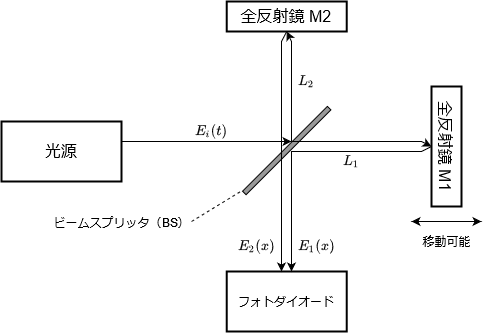
\includegraphics[width = 0.5\textwidth]{画像フォルダ/Interferometer.png}
    \caption{マイケルソン干渉計の構成}
    \label{Michelson_interferometer}
\end{wrapfigure}

光源から射出された光をビームスプリッタ(BS)を用いて二分する。二分したビームの一方は固定反射鏡2へ向かい、もう一方は移動反射鏡M1へ向かう。二分された光は、それぞれM1、M2によって反射して再びBSに戻って合成される。ここで入射光の電場の周波数$\nu$を式\ref{equation_E_i}で表すとする。($a(\nu)$:振幅、$t$:時間)

\begin{equation}
    E_{i}(t) = a(\nu)\exp(i2{\pi\nu}t)
    \label{equation_E_i}
\end{equation}

BSを透過・反射するさいに振幅にかかる係数をそれぞれ$t_{BS}$,$r_{BS}$とし、この瞬間に生じる位相変化をそれぞれ$\delta_{1}$,$\delta_{2}$とする。固定反射鏡M1・移動反射鏡M2から反射し、再びBSに戻ってきた光の電場は、式\ref{equation_E_M1}と式\ref{equation_E_M2}のように示すことができる。

\begin{equation}
    E_{1}(\nu, t) = t_{BS}a(\nu)\exp\left[i\left\{{2{\pi\nu}t-{\frac{2{\pi\nu}L_1}{c}}+\delta_1}\right\}\right] 
    \label{equation_E_M1}
\end{equation}

\begin{equation}
    E_{2}(\nu, t) = r_{BS}a(\nu)\exp\left[i\left\{{2{\pi\nu}t-{\frac{2{\pi\nu}L_2}{c}}+\delta_2}\right\}\right] 
    \label{equation_E_M2}
\end{equation}

$t_{BS}=r_{BS}=1/\sqrt{2}$の時、BSの反射と通過がそれぞれ一度だけ発生した事に留意して、フォトダイオードに入り込む合成光の電場は計算すると、

\begin{equation}
    \begin{split}
    E_{o}&=r_{BS}E_{1}(\nu,t)+t_{BS}E_{2}(\nu,t)\\
    &=\frac{1}{2}a(\nu)\left[\exp \left\{2\pi{i\nu}\left(t-\frac{L_1}{c}\right)+i\delta_1 \right\}+\exp \left\{2\pi{i\nu}\left(t-\frac{L_2}{c}\right)+i\delta_2 \right\} \right] 
    \label{equation_E_o}
    \end{split}
\end{equation}

となる。光強度は振幅の二乗に比例する。よって、合成波の電場の強度は式\ref{equation_E_strength}のように示すことができる。

\begin{equation}
    {\left\lvert E_{o}(\nu, t)\right\rvert} ^2 = \frac{1}{2}a^{2}(\nu)\left\{1+\cos\left(2\pi\nu\frac{L_{1}-L_{2}}{c}+\delta_{2}-\delta_{1}\right) \right\} 
    \label{equation_E_strength}
\end{equation}

ここで$a^{2}(\nu)$は振幅の二乗であり、周波数$\nu$に対する光スペクトル$G(\nu)$である。合成波を受光したフォトダイオードの出力は、$\left\lvert E_{o}\right(\nu,t)\rvert ^2$に比例した電流が発生し、反射鏡M1を移動させて、$L_{1}$を連続的に変化させる事で、$L_{1}$に対して交流的に変化する成分が光強度に含まれることになる。\\
ここで、$\tau=(L_{1}-L_{2}/c)$及び、$\delta=\delta_{2}-\delta_{1}$とすると、光強度は式\ref{equation_E_o_short}のように示せる。

\begin{equation}
    {\left\lvert E_{o}(\nu,t)\right\rvert}^2=\frac{1}{2}G(\nu)\cos(2\pi\nu\tau+\delta)
    \label{equation_E_o_short}
\end{equation}

M1の移動距離を$x$とすると、$\tau=2x/c$となる。

以上の議論により、入射光の光スペクトルが$G(\nu)$である時に発生する交流成分は、式\ref{equation_V}の通りとなる。

\begin{equation}
    V(x)=\int_{0}^{+\infty} G(\nu)\cos\left(\frac{4{\pi}{\nu}x}{c} + \delta\right) \,dx 
    \label{equation_V}
\end{equation}

$G(\nu)$は$V(x)$のフーリエ変換により求めることができる。

\begin{equation}
    G(\nu)=\frac{4}{c} \int_{+\infty}^{-\infty} V(x)\exp\left(\frac{4{\pi}i{\nu}x}{c}\right)  \,dx 
\end{equation}



\section{実験}

\subsection{注意事項}
実験を進める上で、注意すべき点について記述する。

\subsubsection{干渉計}


\subsubsection{光源}

\subsubsection{光ファイバーケーブル}

\subsection{He-Neレーザー光を用いた光干渉}

\subsection{ASE光源の光スペクトル検出}

\section{実験結果}

\subsection{He-Neレーザー光を用いた光干渉実験結果}
オシロスコープで観測した波形をcsv形式で出力した。出力したcsvファイルをExcelを用いて波形を描画した。その波形を図\ref{graphic_day_1}に示す。

\begin{figure}[h]
    \centering
    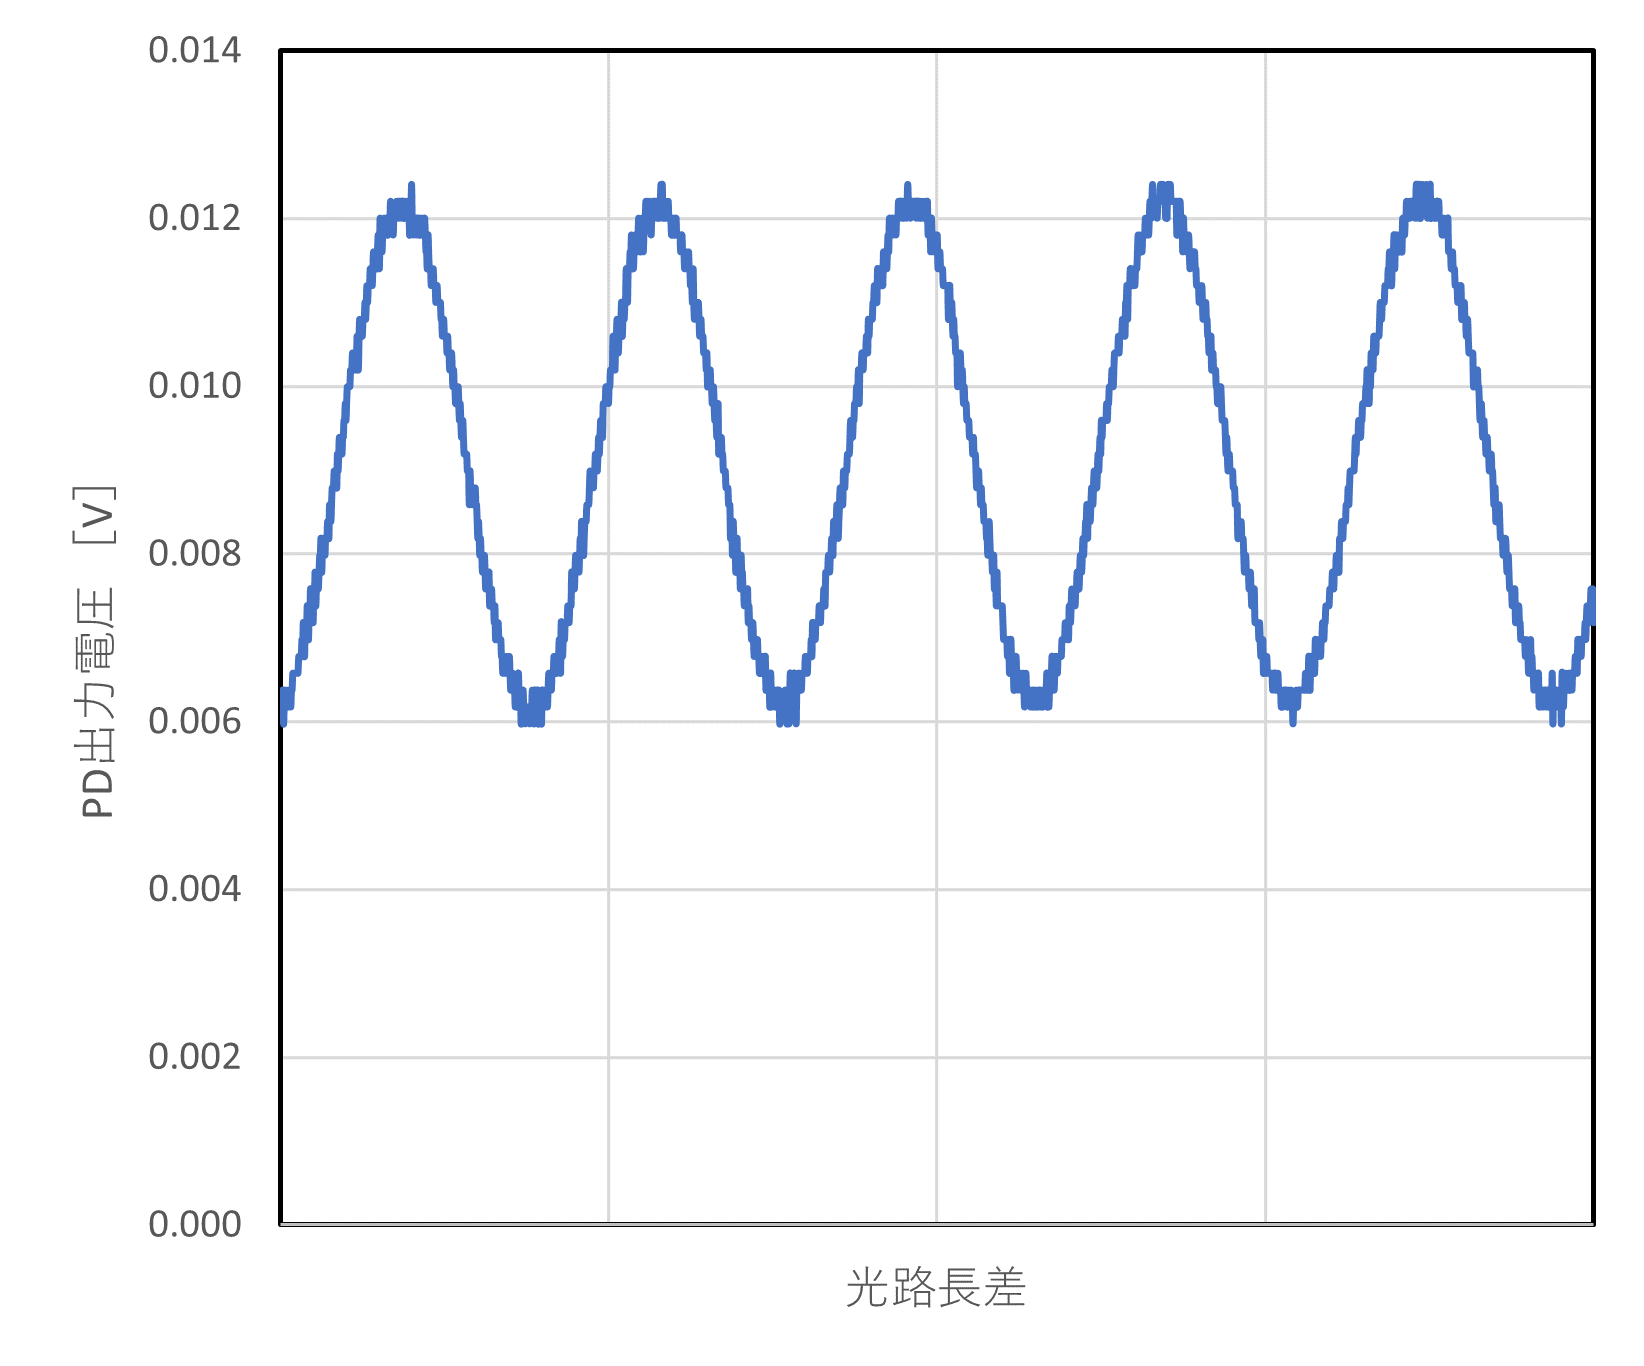
\includegraphics[width = 10cm]{画像フォルダ/wave_day_1.png}
    \caption{He-Neレーザーの光干渉}
    \label{graphic_day_1}
\end{figure}

移動反射鏡M1を移動させることで、光路長が変化しそれに応じて、フォトダイオードに入り込む光強度が周期的に変化していることが見て取れる。

\subsection{ASE光源の光スペクトル検出結果}
波形観測を二回行い、サンプルを二枚作成した。その画像を図\ref{graphics_day_2}に示す。

\begin{figure}[h]
\begin{minipage}{0.5\textwidth}
\centering
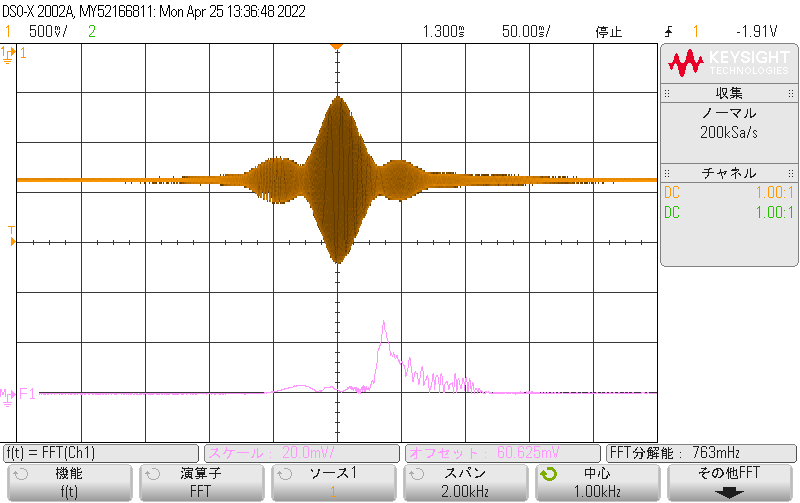
\includegraphics[width = 8cm]{画像フォルダ/scope_1.png}
\subcaption{一回目の波形観測結果}
\label{graphic_day_2_sample_1}
\end{minipage}
\begin{minipage}{0.5\textwidth}
\centering
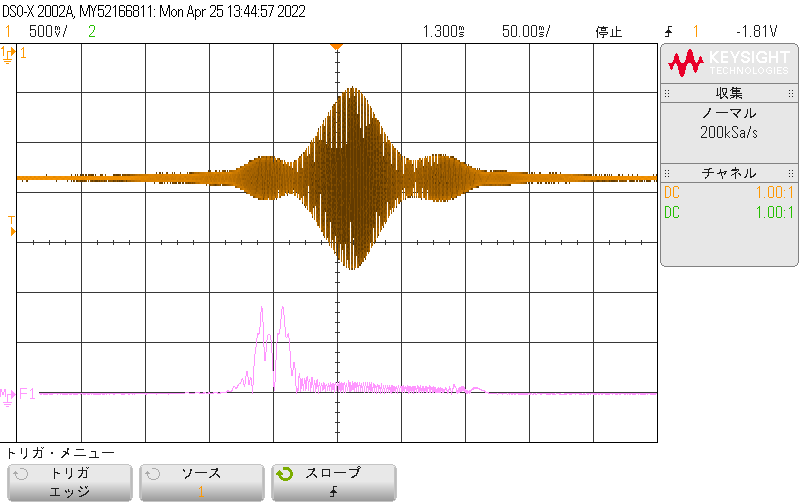
\includegraphics[width = 8cm]{画像フォルダ/scope_2.png}
\subcaption{二回目の波形観測結果}
\label{graphic_day_2_sample_2}
\end{minipage}
\caption{ASE光源の光スペクトル検出結果}
\label{graphics_day_2}
\end{figure}

M1の移動速度に依存して波形がひずむため、不揃いな波形をしている。しかし、概ね同様の波形を観測することができている。

\section{考察}

\subsection{マイケルソン干渉計における光出力強度}
He-Neレーザ光を用いた場合、周期的な信号が観測される。干渉計への入力が一定であることを考えると、エネルギー保存則によってフォトダイオードからの出力は一定でなければならない。しかし、実際にオシロスコープで観測した波形は周期的に変化している。フォトダイオードからの出力が最大でない場合、残りのエネルギーがどのような振る舞いをしたのかを考える。

\begin{wrapfigure}{r}[10pt]{0.5\textwidth}
    \centering
    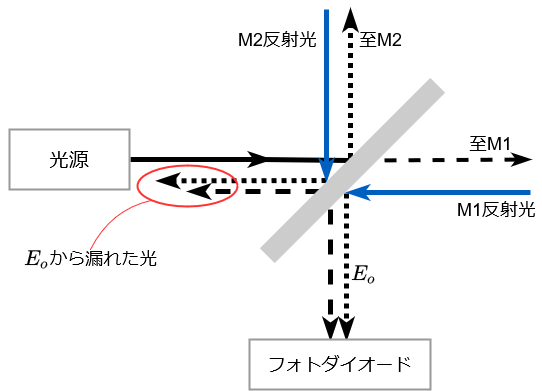
\includegraphics[width = 0.5\textwidth]{画像フォルダ/interference_detail.png}
    \caption{漏れる分の光}
    \label{interferometer_detail}
\end{wrapfigure}

\subsubsection{ビームスプリッタの役割}
式\ref{equation_E_o_short}によると、光強度は$L_{1}$によって周期的に変化することがわかる。そして、$\cos(2\pi\nu\tau+\delta)$が0となるときに、光強度も0となる。しかし、ここで注意するべき点は、\ref{equation_E_o_short}が示す光強度は、フォトダイオードに入り込む光の強度を示している事である。そこで、ビームスプリッタの作用について考える。ビームスプリッタは、光を二分する器具である。それを考慮すると、実際の光の道筋は図\ref{interferometer_detail}に示したような経路を辿っている事になる。この図の細かい点線が反射光、粗い点線が透過光を示している。図\ref{Michelson_interferometer}には、複雑さを回避するため表記を省略している。$L_{1}$を変化させると、M1の反射光とM2の反射光の一部は、BSに当たった際にフォトダイオード側に向かうことなく漏れ出ていく。これが、周期的に光強度が変化する原因である。\cite{wave_and_energy_conservation_law}

\subsection{ミラーの移動速度変動の影響の抑制}
反射鏡M2を波長オーダーの領域で等速で移動させることは難しい。一定の速度で移動しなくても$V(x)$の変化を正確にする方法を考える。

M1の移動とともに現れるビート信号の周期は、$x$の移動分にのみ依存し、レーザー波長の1/2だけ移動した時間がビート信号の周期に相当する。

\subsection{ASE光源の光スペクトルの類推}
図\ref{graphics_day_2}に示した波形を、模した関数を\eqref{equation_V}に示す。

\begin{equation}
    V(\nu)=\exp\left(-\frac{(\nu-\nu_{0})^2}{\sigma^2}\right) \cos\left(\frac{4{\pi}x{(\nu-\nu_{0})}}{\lambda}\right)\cos\left(\frac{\nu-\nu_{0}}{\pi}\right)
    \label{equation_V_function}
\end{equation}

\begin{wrapfigure}{r}[10pt]{0.5\textwidth}
    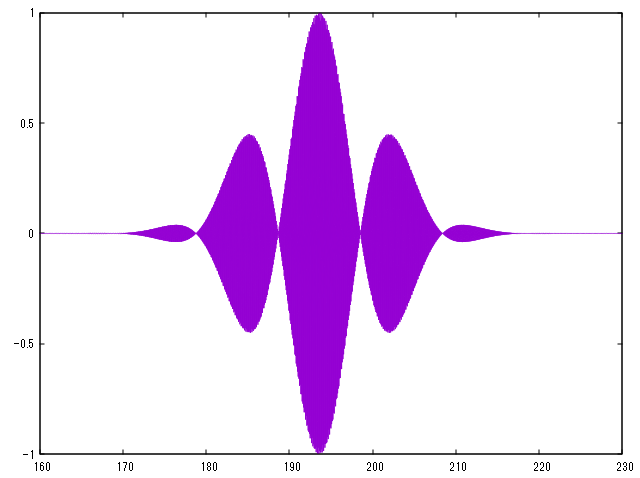
\includegraphics[width = 0.5\textwidth]{画像フォルダ/spector_sample.png}
    \caption{\eqref{equation_V_function}の波形の様子(gnuplotで作成)}
    \label{function_V_sample_wave}
\end{wrapfigure}

$\nu_{0}$は中心周波数で、$\sigma$は$V(\nu)$=1/eとなるときの周波数$\nu$から、中心周波数$\nu_0$を引いた時の絶対値である。

この関数の実際の波形をgnuplotを用いて描画した様子を図\ref{function_V_sample_wave}に示す。横軸は周波数[THz]で、縦軸がパワースペクトル値を表している。このように、波形の積によって図\ref{graphics_day_2}に示したものに似た波形を表現することができる。この時、$\sigma=7.2$,$\nu_{0}$=193.6,x=0.006,$\lambda$=1.55$\times 10^{-6}$として描画を行った。

この関数のスペクトルの概形を推測する。
ここでガウス関数$G(\nu)$のフーリエ変換について考える。ガウス関数$G(\nu)$のフーリエ変換は\eqref{equation_fourier_gauss}の通りとなる。

\begin{equation}
    \mathcal{F}\left[ G(\nu) \right] = \sqrt{\frac{\pi}{\sigma}}\exp\left({-\frac{\nu^2}{4\sigma}}\right)
    \label{equation_fourier_gauss}
\end{equation}

一方、$\cos$は周期関数であるため、離散スペクトルを取る。離散スペクトルはデルタ関数$\delta(\omega)$を用いて表現することができ、\eqref{equation_fourier_cos}のように示せる。\cite{tusin_housiki}

\begin{equation}
    \begin{split}
    &\mathcal{F}\left[\cos\left(\frac{4{\pi}x({\nu-\nu_0})}{\lambda}\right)\right] = \frac{1}{2}\left[\delta\left(\nu-\frac{4{\pi}x}{\lambda}\right)+\delta\left(\nu+\frac{4{\pi}x}{\lambda}\right)\right] \\
    &\mathcal{F}\left[\cos\left(\frac{\nu-\nu_0}{\pi}\right)\right]=\frac{1}{2}\left[\delta\left(\nu-\frac{1}{\pi}\right)+\delta\left(\nu+\frac{1}{\pi}\right)\right]
    \end{split}
    \label{equation_fourier_cos}
\end{equation}

時間領域での積は、周波数領域内では畳み込み積分で表現することができる。\cite{mathema_Fourier}

\begin{equation}
    \mathcal{F}\left[f\cdot g\right] = \frac{1}{2\pi}\mathcal{F}\left[f(t)\right]\ast \mathcal{F}\left[g(t)\right]
\end{equation}

ここで、デルタ関数を$-\infty$から$\infty$まで積分する場合について確認をしておく。デルタ関数$\delta(t)$について一般的に次のような関係が成り立つ。

\begin{equation}
    f(x)=\int_{-\infty}^{\infty } f(\tau)\delta(x-\tau) \,d\tau 
    \label{equation_delta_int}
\end{equation}

これらを踏まえて、\eqref{equation_V_function}のスペクトルを計算する。式\ref{equation_fourier_gauss}、\eqref{equation_fourier_cos}、を用いると、\eqref{equation_V_function}のフーリエ変換は次のように示すことができる。

\begin{multline}
    \mathcal{F}\left[V(\nu)\right] = \frac{1}{2\pi}\int_{-\infty}^{\infty}\sqrt{\frac{\pi}{\sigma}}\exp\left({-\frac{\nu^2}{4\sigma}}\right)\cdot \frac{1}{2} \left\{\left[\delta\left(\nu-\frac{4{\pi}x}{\lambda}-t\right)+\delta\left(\nu+\frac{4{\pi}x}{\lambda}-t\right)\right]\right. \\
    +\left.\left[\delta\left(\nu-\frac{1}{\pi}-t\right)+\delta\left(\nu+\frac{1}{\pi}-t\right)\right]\right\}\,dt
\end{multline}
\begin{multline}
    \qquad \quad =\frac{1}{4\pi}\sqrt{\frac{\pi}{\sigma}}\int_{-\infty}^{\infty}\exp\left({-\frac{\nu^2}{4\sigma}}\right)\left[\delta\left(\nu-\frac{4{\pi}x}{\lambda}-t\right)+\delta\left(\nu+\frac{4{\pi}x}{\lambda}-t\right)\right] \,dt\\
    +\frac{1}{4\pi}\sqrt{\frac{\pi}{\sigma}}\int_{-\infty}^{\infty} \exp\left({-\frac{\nu^2}{4\sigma}}\right) \left[\delta\left(\nu-\frac{1}{\pi}-t\right)+\delta\left(\nu+\frac{1}{\pi}-t\right)\right]\,dt 
    \label{equation_fourier_V}
\end{multline}
\vspace{3mm}
\eqref{equation_delta_int}を用いると、
\begin{equation}
    =\frac{1}{4\pi}\sqrt{\frac{\pi}{\sigma}}\left\{\exp\left(-\frac{(\nu-\frac{4{\pi}x}{\lambda})^2}{4\sigma}\right)+\exp\left(-\frac{(\nu+\frac{4{\pi}x}{\lambda})^2}{4\sigma}\right)+\exp\left(-\frac{(\nu-\frac{1}{\pi})^2}{4\sigma}\right)+\exp\left(-\frac{(\nu+\frac{1}{\pi})^2}{4\sigma}\right)\right\}
    \label{equation_fourier_ans}
\end{equation}

\vspace{3mm}

$\sigma=7.2$,$\nu_{0}$=193.6,x=0.006,$\lambda$=1.55$\times 10^{-6}$とし、gnuplotを用いて、\eqref{equation_fourier_ans}の波形を描画した。横軸周波数[THz]、縦軸をパワースペクトル値とした結果を図\ref{result_spector_wave}に示す。

\begin{figure}[h]
    \centering
    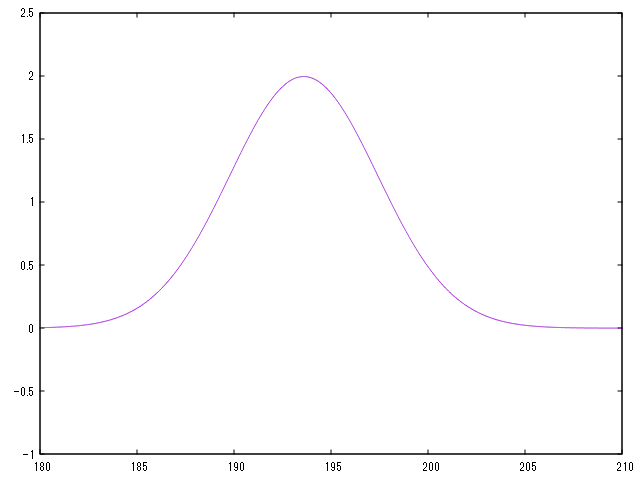
\includegraphics[width = 11cm]{画像フォルダ/result_spector.png}
    \caption{\eqref{equation_fourier_ans}の波形}
    \label{result_spector_wave}
\end{figure}

\subsection{サイドローブの起源}
ASE光源を用いた場合の観測波形$V(x)$には、中央のピークの周りに小さなピーク(サイドローブ)が二つ現れる。このサイドローブが発生する原因について考える。

\subsubsection{ビート信号の解析}
移動反射鏡M1を移動させたときに発生するビート信号$V(x)$は次式で与えられる。

\begin{equation}
    V(x)=\int_{0}^{\infty} \exp\left(\frac{-(\nu-\nu_0)^2}{\sigma}\right)\cos\left(\frac{4{\pi}{\nu}x}{c}\right) \,d\nu
\end{equation}

$V(x)$を解析的に解く。\cite{integral_calculator}

\begin{equation}
    \begin{split}
        V(x)&=\int_{0}^{\infty} \exp\left(\frac{-(\nu-\nu_0)^2}{\sigma}\right)\cos\left(\frac{i4{\pi}x{\nu}}{c}\right) \,d\nu \\
        &=\frac{1}{2}\int_{0}^{\infty} \left\{\exp\left(\frac{i4{\pi}x{\nu}}{c}\right)+\exp\left(-\frac{i4{\pi}x{\nu}}{c}\right)\right\}\exp\left\{-\frac{(\nu-\nu_0)^2}{\sigma^2}\right\} \,d\nu \\
        &=\frac{1}{2}\int_{0}^{\infty} \exp\left(\frac{i4{\pi}x{\nu}}{c}-\frac{(\nu-\nu_0)^2}{\sigma^2}\right) \,d\nu + \frac{1}{2}\int_{0}^{\infty} \exp\left(-\frac{i4{\pi}x{\nu}}{c}-\frac{(\nu-\nu_0)^2}{\sigma^2}\right) \,d\nu \\
        &=\frac{1}{2}\int_{0}^{\infty} \exp\left\{\frac{{\nu}^2}{\sigma^2}+\left(\frac{2\nu_0}{\sigma^2}+\frac{4{\pi}x}{c}i\right)\nu-\frac{{\nu_0}^2}{\sigma^2}\right\} \,dx + \frac{1}{2}\int_{0}^{\infty} \exp\left\{\frac{{\nu}^2}{\sigma^2}+\left(\frac{2\nu_0}{\sigma^2}-\frac{4{\pi}x}{c}i\right)\nu-\frac{{\nu_0}^2}{\sigma^2}\right\} \,dx
    \end{split}
    \label{equation_V_task}
\end{equation}

ここで、第一項と第二項に分けて不定積分を行う。まず、第一項の不定積分$V_1(x)$から求めると、以下のようになる。

\begin{equation}
    V_1(x) = \int \exp\left(\frac{i4{\pi}x{\nu}}{c}-\frac{(\nu-\nu_0)^2}{\sigma^2}\right) \,d\nu =\int \exp\left(-\frac{\nu^2}{\sigma^2}+\left(\frac{i4{\pi}x{\nu}}{c}-\frac{2\nu_0}{\sigma^2}\right)\nu-\frac{(\nu-\nu_0)^2}{\sigma^2}\right) \,d\nu
    \label{equation_V_1_first}
\end{equation}
平方完成すると
\begin{equation}
    =\int \exp\left\{-\left(\frac{x}{\sigma}-\frac{\sigma\left(\frac{i4{\pi}x}{c}+\frac{2\nu_0}{\sigma^2}\right)}{2}\right)^2+\frac{b^2\left(\frac{i4{\pi}x}{c}+\frac{2\nu_0}{\sigma^2}\right)}{4}-\frac{{\nu_0}^2}{\sigma^2}\right\} \,d\nu
\end{equation}
$u=(c\nu-i2{\sigma^2}{\pi}x-{\nu_0}c)/{\sigma}c$を用いて置換積分を行う。よって$\frac{du}{d\nu}=\frac{1}{\sigma}$であるので
\begin{equation}
    \begin{split}
        &=\int \sigma \exp\left\{-\left(u-\sigma\left(\frac{i2{\pi}x}{c}+\frac{\nu_0}{\sigma^2}\right)+\frac{i2{\pi}x{\sigma}^2+{\nu_0}c}{{\sigma}c}\right)^2+\frac{\sigma^2\left(\frac{i4{\pi}x}{c}+\frac{2\nu_0}{\sigma^2}\right)^2}{4}-\frac{{\nu_0}^2}{\sigma^2}\right\} \,du \\
        &=\frac{\sqrt{\pi}\sigma\exp\left(\sigma^2\left(\frac{i2{\pi}x}{c}-\frac{\nu_0}{\sigma^2}\right)-\frac{\nu_0}{\sigma^2}\right)^2-\frac{{\nu_0}^2}{\sigma^2}}{2}\int \frac{2e^{-u^2}}{\sqrt{\pi}} \,du
    \end{split}
\end{equation}

この式を変形する際に、次式に示す関係を用いる。
\begin{equation}
    \frac{2}{\sqrt{\pi}}\int e^{-u^2} \,du = \mathrm{erf}(u) + C_1
\end{equation}
このように定義された関数erf(x)は、誤差関数と名付けられている。この関係を用いて、変形を続けると以下のようになる。

\begin{equation}
    V_1(x)=\frac{\sqrt{\pi}}{2}\cdot \sigma\exp\left\{\sigma^2\left(\frac{i2{\pi}x}{c}+\frac{\nu_0}{\sigma^2}\right)-\frac{{\nu_0}^2}{\sigma^2}\right\} \cdot \mathrm{erf}(u) + C
\end{equation}

忘れずに、$u=(c\nu-i2{\sigma^2}{\pi}x-{\nu_0}c)/{\sigma}c$を代入すると、

\begin{equation}
    V_1(x)=\frac{\sqrt{\pi}}{2}\cdot \sigma\exp\left\{\sigma^2\left(\frac{i2{\pi}x}{c}+\frac{\nu_0}{\sigma^2}\right)-\frac{{\nu_0}^2}{\sigma^2}\right\} \cdot \mathrm{erf}\left(\frac{c\nu-i2{\sigma^2}{\pi}x-{\nu_0}c}{{\sigma}c}\right) + C_1
    \label{equation_V_1_last}
\end{equation}

\eqref{equation_V_1_first}から\eqref{equation_V_1_last}までと同様の手順で、\eqref{equation_V_task}の第二項の不定積分$V_2(x)$を解くと、次式の通りとなる。

\begin{equation}
    V_2(x)=\frac{\sqrt{\pi}}{2}\cdot \sigma\exp\left\{\sigma^2\left(\frac{i2{\pi}x}{c}-\frac{\nu_0}{\sigma^2}\right)-\frac{{\nu_0}^2}{\sigma^2}\right\} \cdot \mathrm{erf}\left(\frac{c\nu+i2{\sigma^2}{\pi}x-{\nu_0}c}{{\sigma}c}\right) + C_2
    \label{equation_V_2_last}
\end{equation}

\eqref{equation_V_1_last}、\eqref{equation_V_2_last}より

\begin{equation}
    \begin{split}
        V(x)&=\frac{1}{2}\int_{0}^{\infty} \exp\left(\frac{i4{\pi}x{\nu}}{c}-\frac{(\nu-\nu_0)^2}{\sigma^2}\right) \,d\nu + \frac{1}{2}\int_{0}^{\infty} \exp\left(-\frac{i4{\pi}x{\nu}}{c}-\frac{(\nu-\nu_0)^2}{\sigma^2}\right) \,d\nu \\
        &=\frac{\sqrt{\pi}}{2} \frac{1}{2}\cdot\sigma\left[\left[\exp\left\{\sigma^2\left(\frac{i2{\pi}x}{c}+\frac{\nu_0}{\sigma^2}\right)-\frac{{\nu_0}^2}{\sigma^2}\right\} \cdot \mathrm{erf}\left(\frac{c\nu-i2{\sigma^2}{\pi}x-{\nu_0}c}{{\sigma}c}\right) \right.\right.\\
        &\qquad\qquad\qquad\qquad\left.\left. + \exp\left\{\sigma^2\left(\frac{i2{\pi}x}{c}-\frac{\nu_0}{\sigma^2}\right)-\frac{{\nu_0}^2}{\sigma^2}\right\} \cdot \mathrm{erf}\left(\frac{c\nu+i2{\sigma^2}{\pi}x-{\nu_0}c}{{\sigma}c}\right)\right]+C\right]_{0}^{\infty}
    \end{split}
\end{equation}

計算すると、次式で与えられる。

\begin{multline}
    V(x)=\frac{\sqrt{\pi}}{4}\sigma \cdot \exp\left(-\frac{4{\pi^2}{\sigma^2}x^2}{c^2}\right)\left\{\left(\cos \left(\frac{4{\pi}{\nu_0}x}{c}\right)+i\sin \left(\frac{4{\pi}{\nu_0}x}{c}\right)\right)\mathrm{erf}\left(\frac{i2{\pi}{\sigma^2}x+{\sigma}c}{{\sigma}c}\right)\right. \\
    +\left(-\cos \left(\frac{4{\pi}{\nu_0}x}{c}\right)+i\sin \left(\frac{4{\pi}{\nu_0}x}{c}\right)\right)\mathrm{erf}\left(\frac{i2{\pi}{\sigma^2}x-{\sigma}c}{{\sigma}c}\right) \\
    +\left.2\cos\left(\frac{4{\pi}{\nu_0}x}{c}\right)\right\}
\end{multline}

\subsubsection{ガウス型スペクトルの場合}
次に、$G(x)$が複数のガウス型スペクトルの和として示される場合の$V(x)$を求める。

\subsection{FT-IRの特徴と今後}

\begin{thebibliography}{99}
    \bibitem{butsuri_sugaku}三井敏之・山崎了『物理数学―ベクトル解析・複素解析・フーリエ解析』日本評論社 9784535806429 pp179,185-186,189
    \bibitem{mathema_Fourier}馬場敬之(2015) 『素晴らしく実力が付くと評判のフーリエ変換 キャンパス・ゼミ2 改訂2』マセマ出版社 9784907165260 pp144-146
    \bibitem{tusin_housiki}守倉正博(2021)『通信方式』オーム社 9784274214738 pp20-21
    \bibitem{wave_and_energy_conservation_law}井上薫 and 山崎正之. "波の重ね合わせの原理とエネルギー保存則." 東海大学紀要工学部 45.2 (2005)
    \bibitem{integral_calculator}David Scherfgen IT Services."Integral Calculator".https://www.integral-calculator.com/,(2022-05-11)
\end{thebibliography}

\end{document}